\begin{appendix}
\section{Appendix}
\label{sec:appendix}

\subsection{Kommerzielle Temperatursensoren}
	\paragraph{Hygrosens TLOG20-BLUE}
		Das ist \textit{NICHT} unsere Lösung.
		\url{http://shop.hygrosens.com/Messsysteme-acma/
			Messsysteme-fuer-Temperatur/Temperaturmesssysteme/
			Temperaturmesssysteme-BLUETOOTH/
			BLUETOOTH-Temperaturmesssystem-20-Kanaele.html}
			{hygrosens.com/TLOG20-BLUE, Zugriff am 16.04.2011}
	\par
	
	\paragraph{Ampedrf BT11}
		Das ist \textit{NICHT} unsere Lösung.
		\url{http://www.ampedrf.com/modules.htm}
		{BT11 Class1, Zugriff am 16.04.2011}
		\url{http://www.ampedrf.com/datasheets/BT11_Datasheet.pdf}
		{BT11 Datasheet}
	\par 

	\paragraph{\$149 Programmable Universal Key Fob Sensor}
		Wir haben uns für das BlueRadios BR-FOB-SEN-LE4.0 Device  entschieden, weil es
		eine komplette und etablierte Lösung für Temperatur, Beschleunigungs- und
		Licht-Messung ist.
		\url{http://www.blueradios.com/BR-FOB-SEN-LE4.0-S2A.pdf}
		{Blueradios BR-FOB-SEN-LE4, Zugriff am 16.04.2011}
		
		\url{http://www.blueradios.com/hardware_sensors.htm}
		{Blueradios BR-FOB-SEN-LE4}
	\par






	\subsubsection{Datenbankinstanzen}
	Anfallende Daten müssen persistent gespeichert werden. Diese Speicherung wird in eine Datenbank durchgeführt. Genauer betrachtet werden die Daten in einer Instanz einer Datenbank gespeichert. Es gilt zu unterscheiden ob eine Instanz einer Datenbank verwendet wird oder mehrere Instanzen verwendet werden und diese synchron gehalten werden.

	\begin{description}
		\item[Eine Instanz] Bei der Verwendung einer Datenbankinstanz gibt es einen zentralen Datenbankserver. Alle Daten werden von dieser Instanz gelesen und geschrieben. Der Vorteil dabei ist, dass alle gespeicherten Daten auf dieser Instanz sofort zur Verfügung stehen. Der Nachteil ist, dass die Datenbank für alle Clients durchgehend zur Verfügung stehen muss.
		\item[Mehrere Instanzen - Jeder synchronisiert mit jedem] Wenn mehrere Instanzen einer Datenbank verwendet werden gilt es diese synchron zu halten. Dies bedeutet, wenn auf einer Instanz Daten erzeugt werden, müssen diese mit anderen Instanzen synchronisiert werden. Eine Möglichkeit ist, dass jede Instanz mit allen anderen Instanzen synchronisiert wird. Dies wäre eine Lösung, wenn es eine definierte Menge von Instanzen gibt und jede Instanz von jeder Instanz aus erreicht werden kann. Dadurch ergibt sich Fehlertoleranz gegenüber Ausfällen von einzelnen Datenbankinstanzen, da die Daten auf jeder Instanz vorliegen und es keine zentrale Masterinstanz gibt.
		\item [Mehrere Instanzen - Jeder synchronisiert mit der Masterinstanz] Anstatt dass jede Instanz mit jeder anderen Instanz synchronisiert wird kann auch eine zentrale Masterinstanz verwendet werden. Diese zentrale Instanz hält alle Daten und verteilt diese Daten wenn nötig auf andere Instanzen. Diese bedeutet wenn eine Clientinstanz neue Daten generiert hat werden diese zur Masterinstanz gesendet und wenn der Client bestimmte Daten benötigt kann er diese bei der Masterinstanz abholen. Dadurch ergibt sich aber ein zentraler Fehlerpunkt. Wenn die Masterinstanz ausfällt ist keine Datenverteilung mehr möglich. 
	\end{description}

	Da beim Roadrunner-Projekt die Daten auf mobilen Geräten erzeugt werden und diese oft auch offline arbeiten, müssen die Daten auf dem Gerät ebenfalls gespeichert werden. Diese Daten werden auf dem Gerät in einer Datenbankinstanz gespeichert. Da es einem mobilen Gerät nicht möglich ist zu allen anderen mobilen Geräten im System Kontakt aufzunehmen wird eine zentrale Masterinstanz verwendet. Auf ein mobiles Gerät werden nur solche Daten gespeichert, die für die Abwicklung der Lieferaufträge benötigt werden.

	\subsubsection{Datenspeicherung}

	Daten können in einer Datenbank auf unterschiedliche Arten gespeichert werden. Dieser Abschnitt beschreibt die unterschiedlichen Speicherungsarten und beschreibt ob diese für das Projekt Roadrunner verwendet werden können.

	\begin{description}
		\item[Relationale Datenbank] In einer relationalen Datenbank werden Daten in einer Tabelle gespeichert. Tabellen werden über PrimaryKey-ForeignKey-Verknüpfungen miteinander in Verbindung gebracht. Ein Eintrag in eine Tabelle, die auf eine andere Tabelle verweist, kann nur durchgeführt werden wenn der Eintrag auf den verweisen wird in der anderen Tabelle existiert. Somit müssten sehr viele Daten auf die mobilen Geräte verteilt werden. Ein Beispiel: Ein Temperatur-Log-Eintrag gehört zu einem Sensor und zu einem Warengut. Das Warengut befindet sich in einem Transportbehälter und muss somit mit diesem Verknüpft werden. Der Transportbehälter hat ein Fahrzeug. Ein Fahrzeug gehört zu einem Fuhrpark usw. Die Verwendung einer relationalen Datenbank auf einem mobilen Gerät wäre nur möglich wenn unterschiedliche Datenbankschemas für die Instanzen der mobilen Geräte und des Masters verwendet werden. 
		\item[Objektorientierte Datenbank] Die Daten werden direkt als Objekte in die Datenbank gespeichert. Da auf den mobilen Geräten aber Java-Objekte bestehen und auf der Webapplikation PHP-Objekte verwendet werden ist diese Lösung nicht ohne intensiven Programmieraufwand für die Konvertierung möglich.
		\item[Dokumentdatenbank] Die Daten werden als Dokumente in die Datenbank gespeichert. Ein Log-Eintrag ist ein Beispiel solch eines Dokumentes. Dokumente sind für sich unabhängige Datensätze die beliebig in einem System verteilt werden können. Dokumente haben Versionsnummern. Anhand der Versionsnummer erkennt eine Datenbankinstanz ob es eine alte Version eines Dokumentes besitzt und kann bei der Masterinstanz eine neue Version des Dokumentes abholen.
	\end{description}

	Bei Roadrunner wird eine verteilte Dokumentdatenbank verwendet. Die verwendete Datenbank verwendet als Dokumentstruktur JSON. Für JSON gibt es eine hohe Integration in Java und PHP und ist somit eine einfach zu verwendende Datenstruktur.





	\subsection{Usecases}

	\subsubsection{Login}

	Ein Fahrer hat im System einen Benutzer. Durch Benutzername und Passwort kann sich der Fahrer auf dem Android-System einloggen. Als Authentifizierungssystem zum Server werden dabei CouchDB-User verwendet. Details zum Authentifizierungssystem sind unter Abschnitt \ref{sec:security}.

	Nach dem Einloggen kann der Fahrer sein Fahrzeug wählen. Das Auswählen des Fahrzeuges ist notwendig, damit das Android-System weiß welche Sensoren auszulesen sind. In Kapitel \ref{sensors} ist beschrieben wie jedes Fahrzeug mit Sensoren ausgestattet wird. 

	In Abbildung \ref{fig:login} ist ersichtlich wie der Loginvorgang durchgeführt wird. Nach dem Loginvorgang versucht das System eine Anfrage für neue Daten an den Server zu senden.  Bei einer aktiven Serververbindung werden die Benutzerdaten und das gewählte Fahrzeug an den Server gesendet. Nach einer Authentifizierung des Benutzers wird ermittelt ob für das gewählte Fahrzeug neue Daten bezüglich der Sensoren vorhanden sind. Sind neue Daten vorhanden werden diese per Datenbankreplikation an das mobile Gerät gesendet.

	Bei der Replikation werden Container-Dokumente übertragen. In diesen Dokumenten sind die Informationen gespeichert, welche Sensoren auf dem jeweiligen Fahrzeug vorhanden sind und wie diese anzusprechen sind.

	\begin{figure}
		\centering
			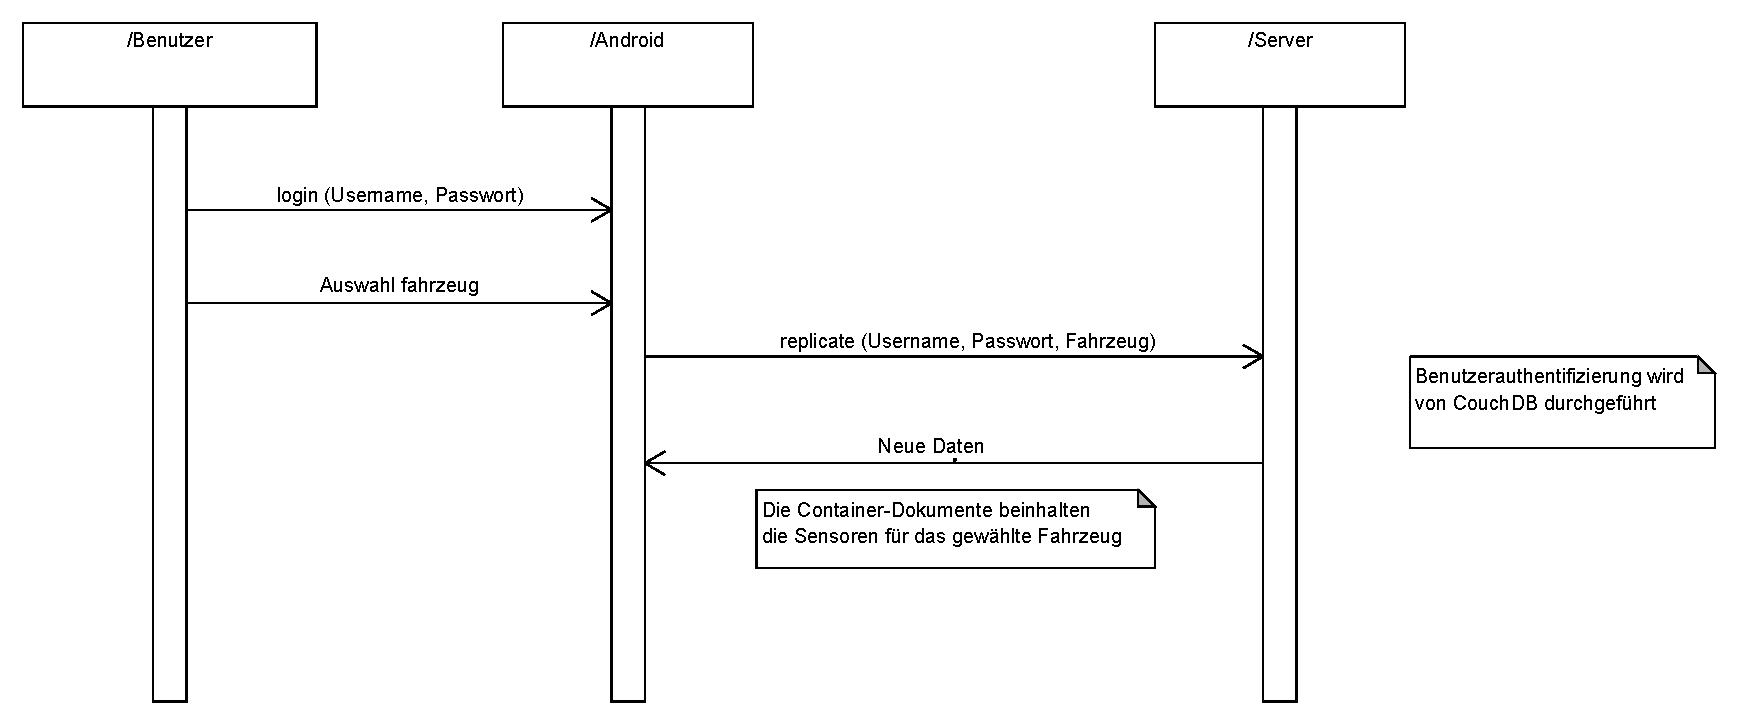
\includegraphics[width=\textwidth]{files/pdf/Login.pdf}
		\caption{Loginvorgang}
		\label{fig:login}
	\end{figure}


	\begin{itemize}
	  \item Wareneingang
	  	\subitem registriert Pakete im System
	  	\subitem klebt QR-Code auf Pakete

		\item Logister plant und erstellt Lieferungen (neue Auftragsnummer wird
		generiert) \subitem wählt Pakete aus (können mit Sensoren bestückt sein)
			\subitem wählt Fahrer aus 
			\subitem wählt Transportmittel (können mit Sensoren bestückt sein) für
			Lieferungen aus
			\subitem trägt Zielort und Auftraggeber ein

	  \item Transporteur
	  	\subitem holt oder hat Device mit Roadrunner App
	  	\subitem loggt sich im Roadrunner System ein
	  		\subsubitem mit Benutzerdaten wird sein/e aktuelle/r Auftrag/Lieferung aufs
	  		Device synchronisiert ODER 
	  		\subsubitem scannt Pakete und lädt sie in das vom Logistiker ausgwählte
	  		Transportmittel
	\end{itemize}

	\paragraph{Daten-Synchronisierung}
		\textbf{Vorbedingungen: }
		\begin{itemize}
		  \item Transporteur hat sich in der System-App eingeloggt
		\end{itemize}

		Die Daten-Synchronisierung oder Replizierung wird durch das Einloggen im
		System angestoßen. Das mobile Gerät erhält folgende Information:
		\begin{itemize}
		  \item Adressen der Sensoren, die das Gerät überwachen sollte
		  \item alle Produkte, Pakete der aktuellen Lieferung, sowie Zielort, etc.
		  \item Überwachungs-Thresholds der Pakete
		\end{itemize}
	\par



	
\end{appendix}
